

\actTitle{Worksheet 3.4}


\noindent \textbf{Instructions:}  Work together in groups of  3 or 4 to complete the following problems.

\noindent CAUTION: There is NO RULE for breaking down $\log_a(u+w)$ or $\log_a(u-w)$.  

Student goals:
\begin{itemize}
\item Use the properties of logarithms to solve for a variable in a
  variety of more complex forms:
  \begin{eqnarray*}
    \log_a(u\cdot v) & = & \log_a(u) + \log_a(v), \\
    \log_a\left(\frac{u}{v}\right) & = & \log_a(u) - \log_a(v), \\
    \log_a\left(u^r\right) & = & r\log_a(u).
  \end{eqnarray*}
\item Solve for a variable when multiple logarithms with different
  bases are present in an expression.
\item Solve for a variable when multiple exponentials with different
  bases are present in an expression.
\end{itemize}

\hrule

\begin{enumerate}

\item Let $M=\log_b(x)$ and $N=\log_b(y)$.
\begin{enumerate}
\item Write the given equations in exponential form.

  \vfill
\item Show that $xy=b^{M+N}$.

  \vfill
\item Write the expression $xy=b^{M+N}$ in logarithmic form.

  \vfill

\item Substitute for $M$ and $N$.

  \vfill
  
\item What did you just show?

  \vspace{1em}

\end{enumerate}

\clearpage

\item Let $M=\log_b(x)$ and $N=\log_b(y)$.  Use the same process as
  that in the previous question to show the Quotient Property of
  Logarithms is true.
  $$\log_b\left(\frac{x}{y}\right)=\log_b(x)-\log_b(y)$$
\vfill
\vfill
\vfill


\clearpage

\item Expand the following to express in terms of logarithms of $x$, $y$, $z$, or $w$.
\begin{enumerate}
\item $\log_4(xz)$ \\[.2in]
%\item $\ln(\sqrt[7]{x^5})$
\item $\log_2\left( \dfrac{x}{y} \right)$ \\[.2in]
\item $\ln\left( \dfrac{w^2z^3}{y^2\sqrt[5]{x}} \right)$ \\[1in]
%\item $\log(z \sqrt[5]{x^7y^3})$
\end{enumerate}



\item Condense the following to express as a single logarithm.
\begin{enumerate}
%\item $\log_3(x)+\log_3(4y^2)$
\item $\log_7(4x^5)-\log_7(x^2)$ \\[.5in]
\item $-4\left(\ln(2)-\ln(7)\right)+5\ln(3)$ \\[.7in]
\item $7 \log_8 (x) - 3 \log_8(2x+3) + 2\log_8(x-3)$ \\[1in]
%\item  $\dfrac{1}{4} \ln(x y^2) + \dfrac{1}{3} \ln(y^5 \sqrt{x} )-3\ln\left(\dfrac{z}{y}\right)$

\end{enumerate}




\clearpage


\item Rewrite the function into an equivalent form without using any
  logarithms.
\begin{enumerate}
\item $ \displaystyle f(x) = 10 \ln(e^{-7+2x})$ \\[.5in]
\item $\displaystyle f(x)=3^{\log_3(8)-5 \log_3(x^2+1)}$ \\[1in]

\item $f(x) = \log ({10}^{4x+y}{100}^{y-x})$ \\[1in]
\end{enumerate}


\item Use the given approximations to approximate the value of the following logarithms.
$$\log_b(2)\approx 0.356 \quad \quad \quad \quad \log_b(3)\approx 0.565 \quad \quad \quad \quad \log_b(5)\approx 0.827$$

\begin{enumerate}
\item $\log_b(15)$\vfill
\item $\log_b(10)$\vfill
\item $\log_b(81)$\vfill
\item $\displaystyle \log_b\left(\frac{15}{2}\right)$\vfill
\end{enumerate}




\clearpage

\item  For each of the following functions, determine whether or not its graph is shown below.

\begin{multicols}{3}
\begin{enumerate}
	\item $y=2^x+3$
	\item $y=\ln(x-2)$
	\item $y = 2^{-x}+3$
	\item $y=e^{-x}-3$
	\item $y=-\ln(x-2)$
	\item $y=-\log_2(x+3)-4$
\end{enumerate}	
\end{multicols}


\begin{center}
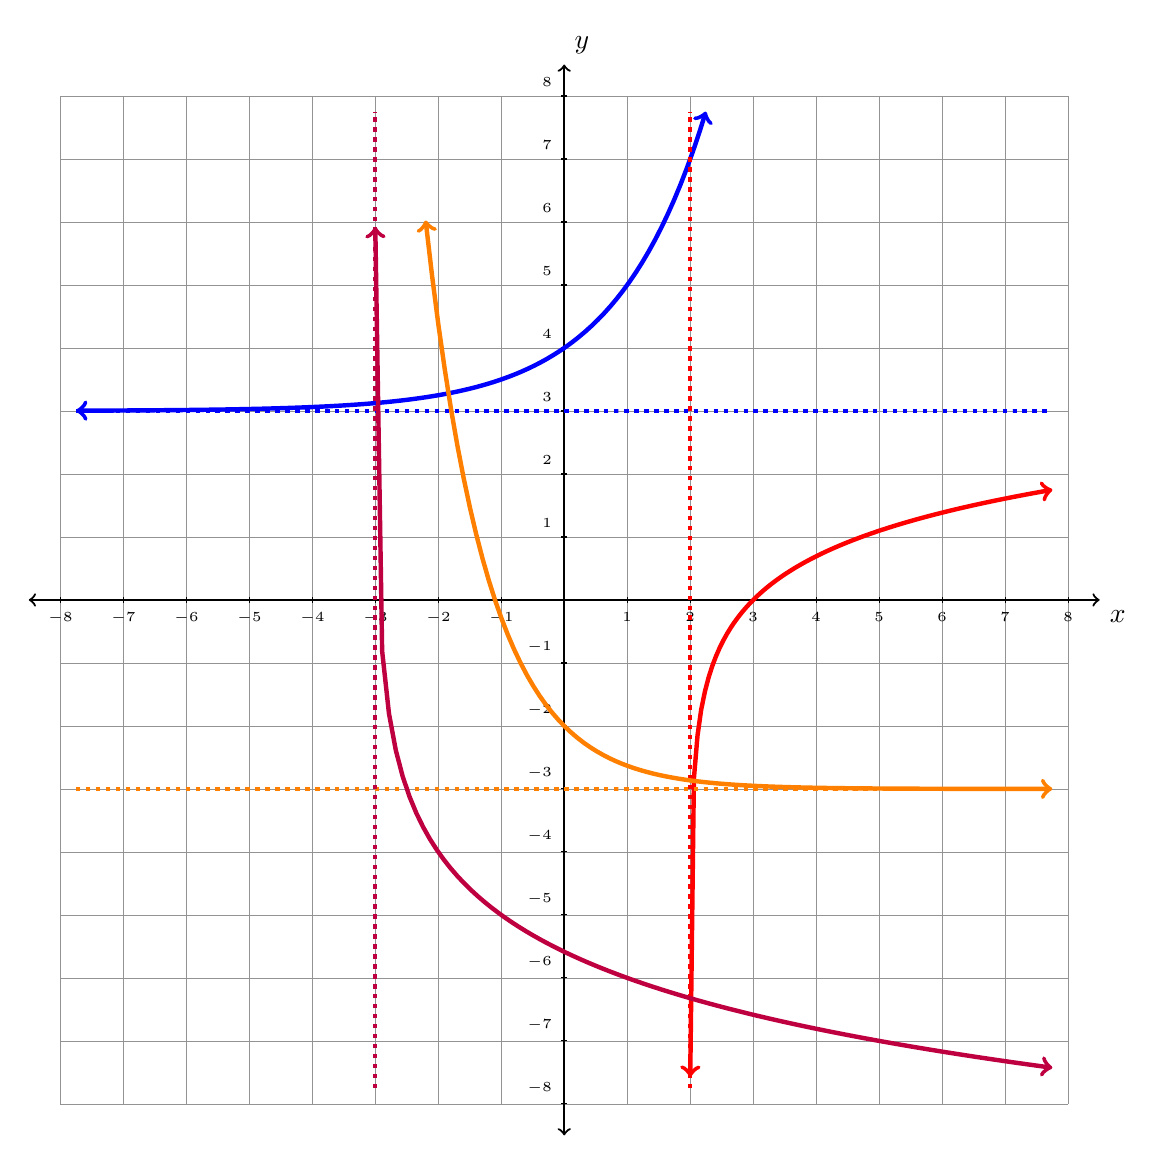
\begin{tikzpicture}[y=.8cm, x=.8cm,font=\sffamily,
	mydot/.style={
    circle,
    fill=white,
    draw,
    outer sep=0pt,
    inner sep=1.5pt
  }]
    %% Add a grid
    \draw[step = 1, gray, very thin,opacity=0.85] (-8, -8) grid (8, 8);
 	%% Draw the axes
	\draw[thick,<->] (-8.5,0) -- coordinate (x axis mid) (8.5,0) node[anchor = north west] {$x$};
    \draw[thick,<->] (0,-8.5) -- coordinate (y axis mid) (0,8.5) node[anchor = south west] {$y$};
    %% Label the y axis
    \foreach \y in {-8,...,-1,1,2,...,8} {
      \draw (1pt, \y) -- (-1pt, \y) node[anchor = south east] {\tiny $\y$};
    }
    %% Label the x axis
    \foreach \x in {-8,...,-1,1,2,...,8} {
      \draw (\x,1pt) -- (\x,-1pt) node[anchor = north] {\tiny $\x$};
    }
    %% Draw the function.
    \begin{scope}
%         \draw[very thick,blue] (-3,2) -- (1,1);
%         \draw[very thick,blue] (3.05,1.05) -- (4,3);
%         \draw[very thick,blue] (1.1,4) -- (3,4);
    %semi-circle
         %\draw[very thick, blue] (1,1) arc [radius=1, start angle=180, end angle= 5];
     %parabola
         %\draw[ultra thick, blue, domain=-5:0] plot (\x, {(-0.2)*(\x-5)*(\x+5)});
         \draw[ultra thick, blue, <->, domain=-7.75:2.25] plot[samples=100] (\x, {2^\x+3});
         \draw[ultra thick, blue, dotted, domain=-7.75:7.75] plot[samples=100] (\x, 3);
         \draw[ultra thick, red, <->, domain=2.0005:7.75] plot[samples=100] (\x, {ln(\x-2)});
         \draw[ultra thick, red, dotted, range=-7.75:7.75] plot[samples=100] (2,-7.75)--(2,7.75);
         \draw[ultra thick, orange, <->, domain=-2.2:7.75] plot[samples=100] (\x, {e^-\x-3});
         \draw[ultra thick, orange, dotted, domain=-7.75:7.75] plot[samples=100] (\x, -3);
         \draw[ultra thick, purple, <->, domain=-2.999:7.75] plot[samples=100] (\x, {-log2(\x+3)-4});
         \draw[ultra thick, purple, dotted, range=-7.75:7.75] plot[samples=100] (-3,-7.75)--(-3,7.75);

           %dots
%         \fill[blue] (-3, 2) circle[radius=0.5ex];
%         \fill[blue] (1,1) circle[radius=0.5ex];
%         \fill[blue] (4,3) circle[radius=0.5ex];
%         \draw[very thick, blue] (3,1) circle[radius=0.5ex];
%         \fill[blue] (3,4) circle[radius=0.5ex];
%         \draw[very thick, blue] (1,4) circle[radius=0.5ex];


    \end{scope}

    %%\node[above=0.1cm] at (-2,2 )   {\nextXValue};

\end{tikzpicture}
\end{center}





\item Use the change-of-base formula to write $\log_2(6)\log_6(7)$ as
  a single logarithm.

  \vfill




\end{enumerate}

\hwTitle{Section 3.4}


\begin{enumerate}
\item For each expression below, condense the left hand side into a
  single logarithm, and then use the definition of the logarithm to
  determine all possible values of $x$ that satisfy the original
  expression.
  \sideNote{Check your answers with the original equation to ensure
    that your solutions are valid.}
  \begin{enumerate}
  \item ${\displaystyle \log(x+2) + \log(x) = 2}$
  \item ${\displaystyle \log(x+2) - \log(x) = 2}$
  \item ${\displaystyle \log(x-3) + \log(x-5) = 1}$
  \item ${\displaystyle \log(2-x)+\log(x+1) = 0 }$
  \end{enumerate}
\item Use the change-of-base formula to write $\log_4(3)+\log_5(7)$ as
  a single logarithm using base $e$.
\item The function $Pm$ is defined by
  \begin{eqnarray*}
    Pm(x) & = & A + B \ln(x).
  \end{eqnarray*}
  It is known that $Pm(1) = 5$ and $Pm(3)=2$. Determine the values of
  $A$ and $B$. What is the long term behaviour of the function?
\item Make a rough sketch of the graphs of $\ln(|x|)$ and
  $\ln(x)$. Briefly describe the differences between them. How do the
  two graphs relate to the graph of $\frac{1}{2}\ln\left(x^2\right)$?
\item For what values of $x$ are the functions $g(x)=2\ln(x)$
  and $h(x)=\ln\left(x^2\right)$ equivalent? Make a rough sketch of
  the two functions.
\item Determine the domain of the function
  \begin{eqnarray*}
    b(x) & = & \ln\left(-x^2+3x-2\right)
  \end{eqnarray*}
  two different ways. First, determine values of $x$ so that the
  quadratic is positive. Second factor the quadratic and use the
  properties of the logarithm to express the function in a different
  form.
\item Determine the approximate numerical values of the expressions
  below given
  \begin{equation*}
    \begin{array}{rcl@{\hspace{2em}}rcl@{\hspace{2em}}rcl}
      \log_b(x) & \approx & -0.4511,&
      \log_b(8) & \approx & 0.6727,&
      \log_b(12) & \approx & 0.8039.
    \end{array}
  \end{equation*}
  \begin{enumerate}
  \item ${\displaystyle \log_b\left(\frac{x}{12} \right) }$
  \item ${\displaystyle \log_b\left(\frac{64\sqrt{x}}{12} \right) }$
  \item ${\displaystyle \log_b\left(\frac{ \sqrt[3]{8} \, x^2 }{144} \right) }$
  \item ${\displaystyle \log_b\left(\frac{2x}{3} \right) }$
  \end{enumerate}
\end{enumerate}
